\documentclass[12pt]{report}
\usepackage{makeidx}
\usepackage{graphicx}
\usepackage{xcolor}
\usepackage{listings}
\usepackage{float}
\usepackage{minted}
\usepackage[left=2cm,right=2cm,top=2cm,bottom=5cm]{geometry}
\usepackage{soul}
\usepackage{array}
\def\mystrut(#1,#2){\vrule height #1 depth #2 width 0pt}
\newcolumntype{C}[1]{%
   >{\mystrut(3ex,2ex)\centering}%
   p{#1}%
   <{}}
\textwidth 6in
\textheight 9in
\topmargin 0in
\headsep 0in
\oddsidemargin 0.5cm
\evensidemargin -0.5cm

\lstset{basicstyle=\ttfamily,
  showstringspaces=false,
  commentstyle=\color{red},
  keywordstyle=\color{blue}
}

\title{Skyscrapers Puzzle with\\
Altera FPGA DE1}

\date{\vspace{-5ex}}

\begin{document}
\author{Students: Andrea Giardini - Francesco Venturoli}
\maketitle

\chapter*{Aim of the project}

The project aim is to write a software to run the Skyscrapers puzzle on
a Altera DE1 board, allowing users to interact with it using the keyboard.
The final result will be an interactive logic puzzle, where the user can
input digits in the game or solve it automatically. The game needs to
recognize when the puzzle is completed and if the solution provided is
correct and satisfies all the constraints.

\begin{figure}[H]
  \centering
  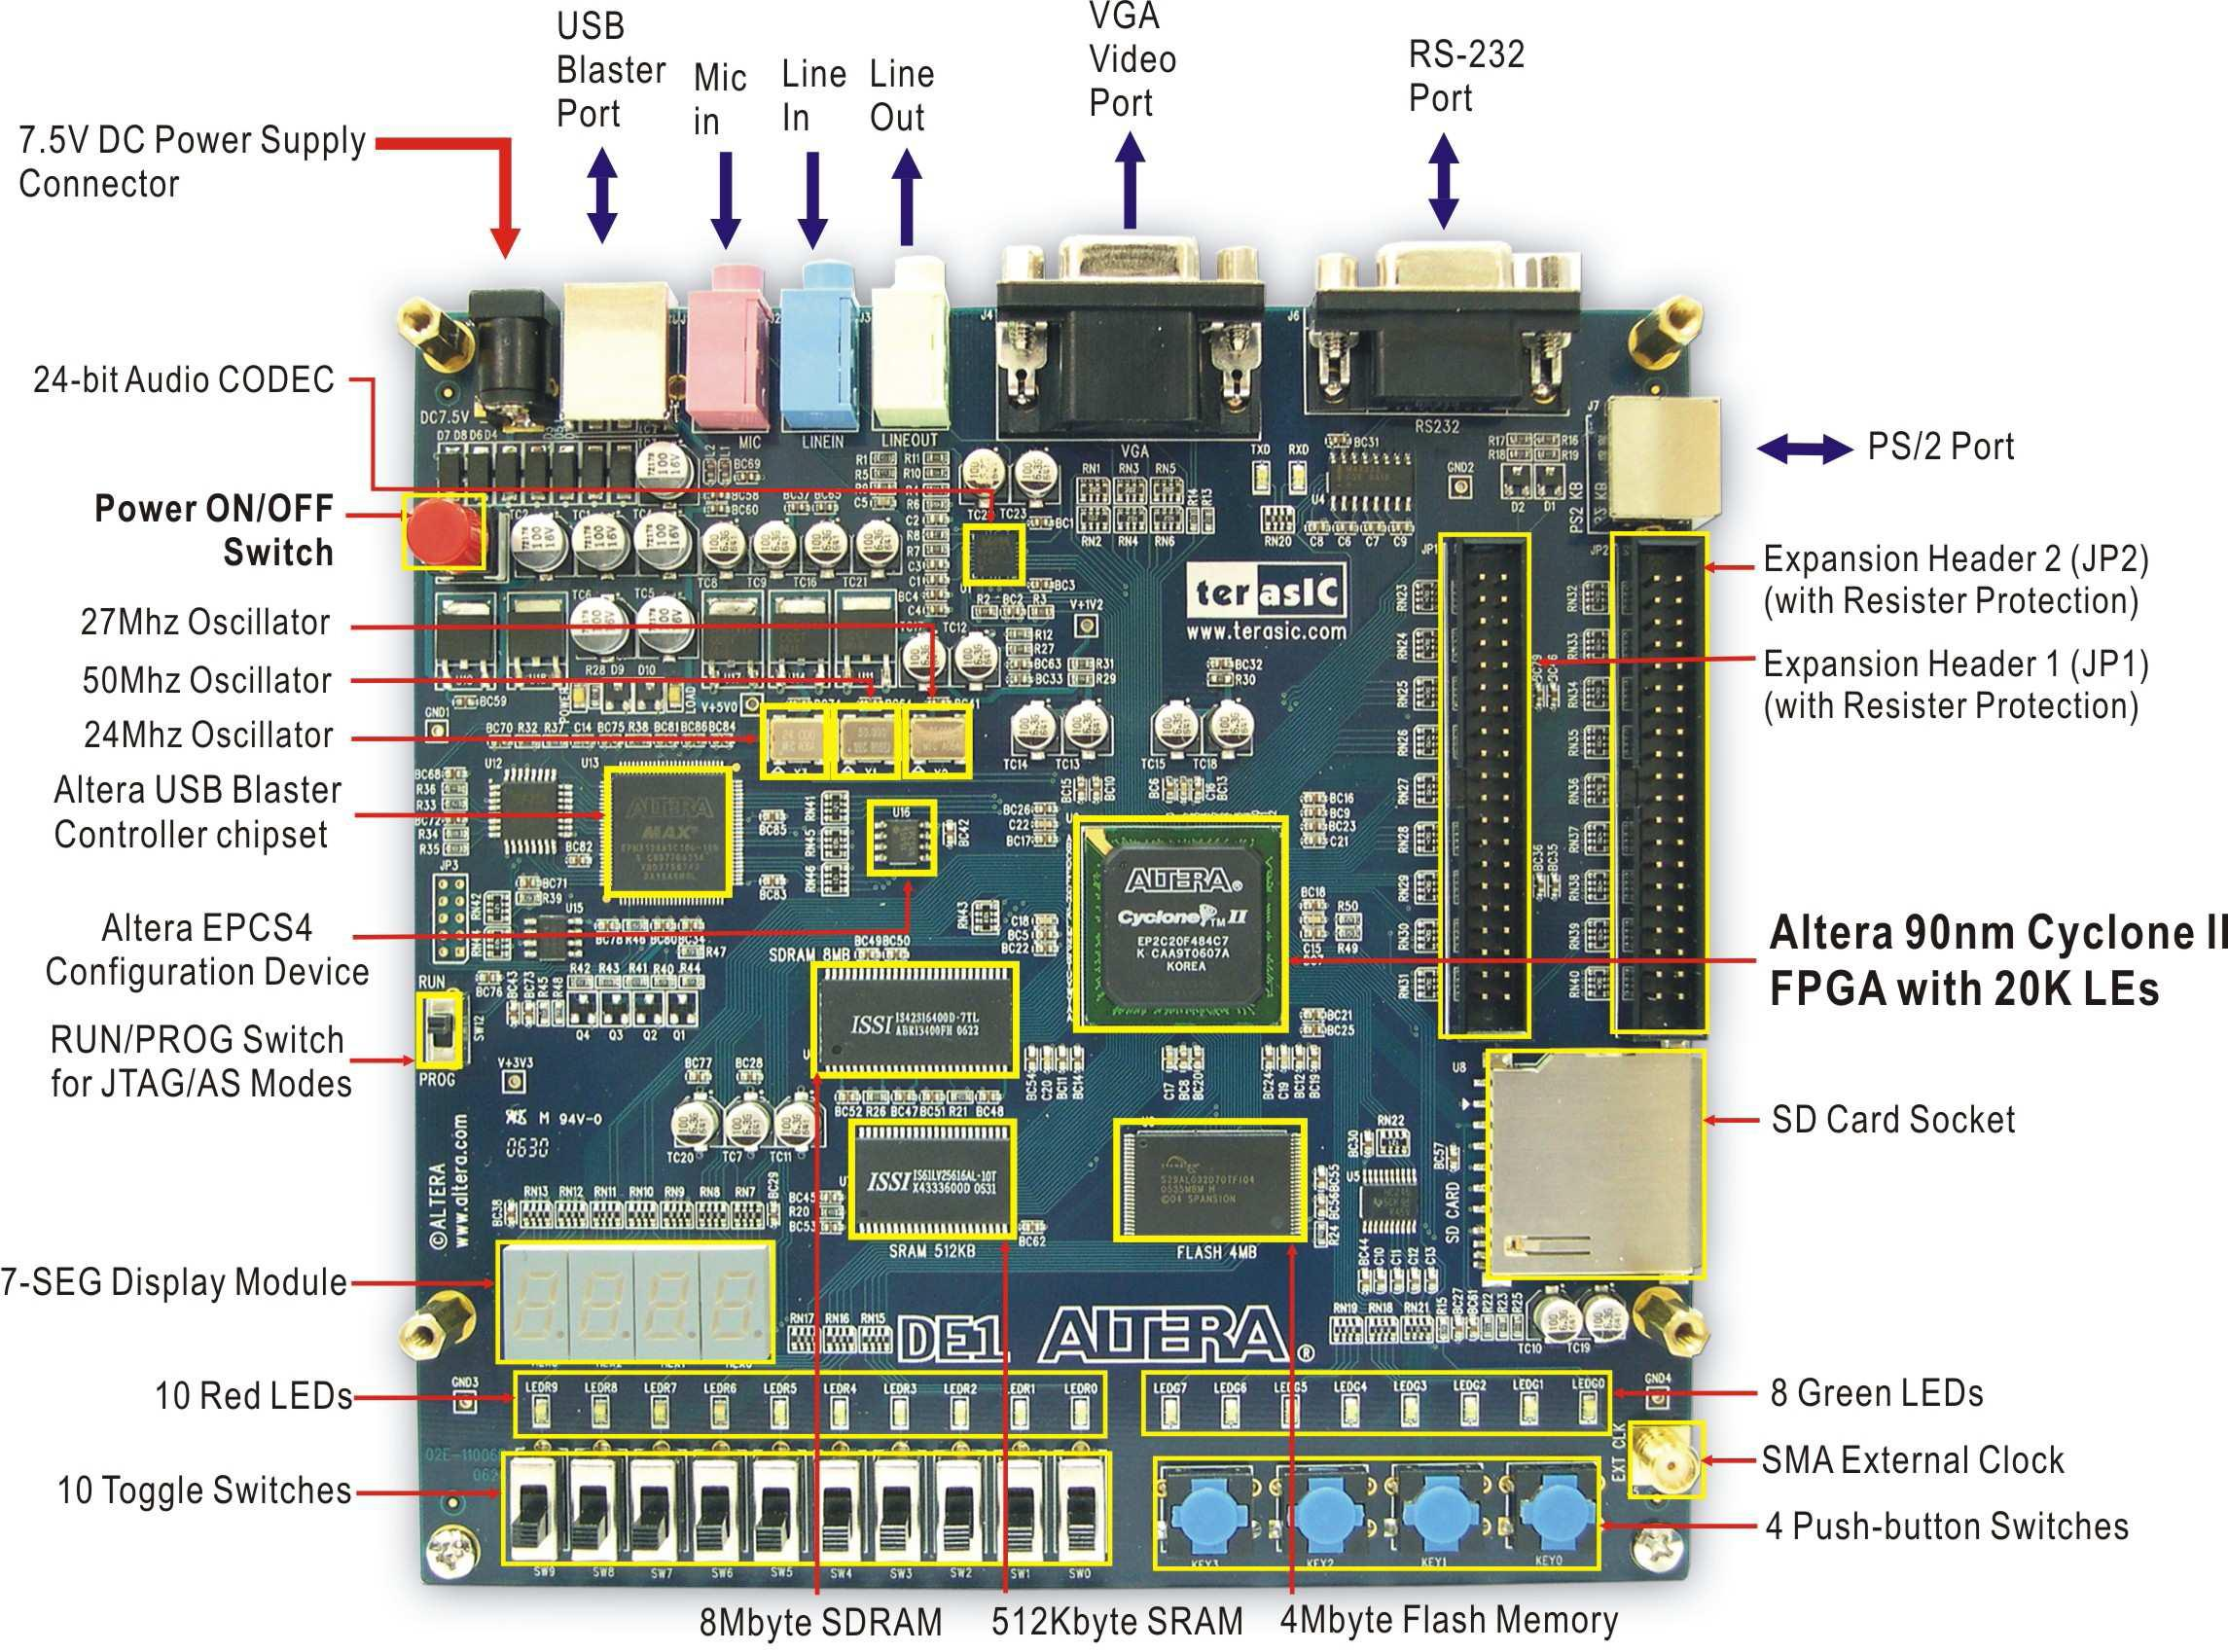
\includegraphics[keepaspectratio,width=0.8\textwidth]{images/Altera_DE1_Board.jpg}
  \caption{Altera DE1 FPGA Board}
\end{figure}

In the proposed game, the user needs to be able to move the cursor in the
matrix using the arrows on the keyboard. Entering numbers in the matrix,
always using the keyboard, the user tries to complete the puzzle filling
all the blank spaces with a numeric value. If the user is not able to
complete the game, the puzzle can automatically be solved by the
algorithm implemented in the board. Once the puzzle is solved, the board
should recognize the solution and show the user that he won.

\chapter*{Introduction to the puzzle}

Each puzzle consists of an NxN grid, organized as a latin square, with some
clues along its sides. The goal is to place a skyscraper in each square,
with a height between 1 and N, so that no two skyscrapers in the same row
or column have the same number of floors. In addition, the number of visible
skyscrapers, as viewed from the direction of each clue, is equal to the value
of the clue. Note that higher skyscrapers block the view of lower skyscrapers
located behind them.

\begin{figure}[H]
  \centering
  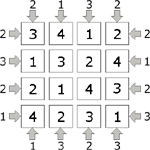
\includegraphics[keepaspectratio]{images/skyscrapers_small_solved.jpg}
  \caption{Solved 4x4 Skyscrapers puzzle}
\end{figure}

There are a number of intuitions that can be addressed immediately,
filling some of the empty spaces with values, while other spaces need
a combination of more constraints to identify the correct value. The game
can be extended with a bigger matrix or to include parks (empty spaces,
represented by buildings with zero height in the matrix). For this project, we
decided to solve the classic version of the puzzle, a 4x4 matrix with no parks.

\newpage

\section*{Control Unit}

The control unit is used in this project to get the inputs from the user
and interpret them. Following that, the interpreted signals are sent to
the Datapath.

As we specified previously, our intention is to let the user use
a keyboard to play the game. In order to do this we have to read the
serial PS2 line and map the received data with the scan codes of the
keys that we want to interpret.

In order to simplify this task and keep the Control Unit as clean as possible,
we added a new class called \textit{Skyscrapers\_Puzzle\_Keyboard}, which
is responsible exclusively of reading the data from the keyboard and mapit
to the corresponding scan codes. Using this class we can leave all the
logic of translating the signals to actions to the Control Unit, as it is
supposed to be.

The Control Unit uses the following signals:

\begin{center}
\begin{minipage}{0.5\textwidth}
\begin{minted}{vhdl}
  CLOCK        : in std_logic;
  keyboardData : in std_logic_vector (7 downto 0);
  RESET_N      : in std_logic;
  TIME_10MS    : in std_logic;

  CURSOR_POS   : in CURSOR_POS_TYPE;

  -- Connections with Data-Path
  MOVE_RIGHT   : out std_logic;
  MOVE_LEFT    : out std_logic;
  MOVE_DOWN    : out std_logic;
  MOVE_UP      : out std_logic;
  NUMBER       : out std_logic_vector (3 downto 0);
  SOLVE        : out std_logic;
  CLEAN        : out std_logic;
\end{minted}
%\caption{Input and Output signals for Control Unit}
\end{minipage}
\end{center}

The Control Unit reads the serial line \textit{keyboardData} and
translates the scan codes received to actions, that are then sent to the
Datapath. In order to avoid reading a single keypress as multiple
keypresses ( since the data clock is too fast ) we are scanning the line
periodically and not constantly.

\newpage

\section*{Datapath}

The Datapath takes care of the logic of the game, it maintains in memory
the numbers that the user added to the matrix. The user is able to add new
numbers to the matrix using the keyboard and all its changes are registered
inside the Datapath. Moreover, the Datapath contains all the logic needed to
solve the puzzle automatically.

\begin{center}
\begin{minipage}{0.5\textwidth}
\begin{minted}{vhdl}
  CLOCK       : in std_logic;
  RESET_N     : in std_logic;
  MOVE_RIGHT  : in std_logic;
  MOVE_LEFT   : in std_logic;
  MOVE_DOWN   : in std_logic;
  MOVE_UP     : in std_logic;
  SOLVE       : in std_logic;
  CLEAN       : in std_logic;

  KEYS        : in std_logic_vector (3 downto 0);

  MATRIX      : out MATRIX_TYPE;
  CONSTRAINTS : out CONSTRAINTS_TYPE;
  SOLUTIONS   : out SOLUTIONS_TYPE;
  CURSOR_POS  : out CURSOR_POS_TYPE;
  WINNER      : out std_logic
\end{minted}
%\caption{Input and Output signals for Datapath}
\end{minipage}
\end{center}

The Datapath is the main component of the project since it stores the
matrix with the values, handles the inputs received from the Controller
and contains the algorithm used to solve the puzzle.

Every cell in the schema is mapped as an array of N logic values (effectively
mapping the game to a NxNxN matrix), each one representing the feasibility
of a solution in a given cell. At the beginning of the game, all values
are feasible in any cell.

When the user inputs a number or invokes the automatic solver, no values are
set in the matrix: instead, other values are deemed infeasible, and thus
removed from the list of feasible values. After this, if a cell is left
with only one feasible solution, its value is assigned to it and displayed
on screen.

\newpage

\section*{View}

The View is responsible for drawing on screen the elements of the Datapath
and represent them in the best way for the user. In our case, the visual
representation of the game is quite simple, but there were some challenges
to be solved, especially with the drawing of numbers.

\begin{center}
\begin{minipage}{0.5\textwidth}
\begin{minted}{vhdl}
  CLOCK        : in std_logic;
  RESET_N      : in std_logic;

  MATRIX       : in MATRIX_TYPE;
  SOLUTIONS    : in SOLUTIONS_TYPE;
  CONSTRAINTS  : in CONSTRAINTS_TYPE;
  CURSOR_POS   : in CURSOR_POS_TYPE;

  REDRAW       : in  std_logic;

  FB_READY     : in  std_logic;
  FB_CLEAR     : out std_logic;
  FB_DRAW_RECT : out std_logic;
  FB_DRAW_LINE : out std_logic;
  FB_FILL_RECT : out std_logic;
  FB_FLIP      : out std_logic;
  FB_COLOR     : out color_type;
  FB_X0        : out xy_coord_type;
  FB_Y0        : out xy_coord_type;
  FB_X1        : out xy_coord_type;
  FB_Y1        : out xy_coord_type;
  HEX0         : out std_logic_vector (6 downto 0);
  HEX1         : out std_logic_vector (6 downto 0);
  HEX2         : out std_logic_vector (6 downto 0);
  HEX3         : out std_logic_vector (6 downto 0)
\end{minted}
%\caption{Input and Output signals for View}
\end{minipage}
\end{center}

As we can see from the signals, we used the FrameBuffer technology to draw
the frames of the game before printing them on the screen. The FrameBuffer
is a portion of memory containing a Bitmap that is used to refresh a video
display from a memory buffer containing a complete frame of data.
Basically what happens is that we draw the whole frame to be displayed in
memory before we display it on video. Once the frame is ready to
be displayed and all the drawing operations are completed, we refresh the
screen, drawing on it the new frame that we just created in memory.

\newpage

The View is organized in different macro states:

\begin{minted}{vhdl}
type state_type is (IDLE, WAIT_FOR_READY, DRAWING);
\end{minted}

In particular we will analyse the DRAWING state, which is made of a set of
sub-states:

\begin{minted}{vhdl}
type substate_type is (CLEAR_SCENE, DRAW_BOARD_OUTLINE, DRAW_BOARD_BLOCKS,
     DRAW_BOARD_CONSTRAINTS, DRAW_BOARD_NUMBERS, FLIP_FRAMEBUFFER);
\end{minted}

Every state draws a different object:

\begin{itemize}
  \item CLEAR\_SCENE

  Cleans the frame in memory, filling it with a black square which will be
  the background of our game.

  \item DRAW\_BOARD\_OUTLINE

  Draws the outline of our game board, just the perimetral square.

  \item DRAW\_BOARD\_BLOCKS

  Draws the blocks inside our game board and the position of the cursor.

  \item DRAW\_BOARD\_CONSTRAINTS

  Draws the constraints around our game board.

  \item DRAW\_BOARD\_NUMBERS

  Draws the numbers that have been inserted inside the board.

  \item FLIP\_FRAMEBUFFER

  This state is reached when the drawing has been completed and we are
  ready to display it on the screen. After this, we go back to IDLE state,
  preparing for the creation of a new frame to display.
\end{itemize}

The most difficult part was drawing the numbers on screen, since the
FrameBuffer library was not giving us any possibility of drawing custom
images but only squares. To draw the numbers we had to define every digit
as a sprite, which is an array of colors, representing pixel by pixel the
color that has to be drawn, considering black as a background color and
white as foreground. After that we had to draw a square of 1x1 pixel for
each pixel of the number's sprite.

\chapter*{Solving algorithm}

In order to solve the puzzle we had to implement in VHDL multiple methods
to remove solutions from the board based on the constraints of the game. In
the following section we will analyze the rules that we are applying to
solve the problem and how they help us to remove infeasible solutions from
the puzzle.

Starting with the structure, we represented the puzzle as
a three-dimensional matrix. This matrix has dimensions 4 (length)
x 4 (height) x 4 (possible solutions). We must consider that, when
a number is inserted, that solution can be removed from the corresponding
row and column, since we cannot have the same number twice on the same
column or row.

During the analysis phase we determined that the most convenient technique
to set the correct value for a cell is to remove all the incorrect values
from the set of possible solutions. This way, when a cell has only
a possible value, we set that value.

\section*{Simple solvers}

\begin{itemize}

    \item \ul{If the constraint is \textbf{one}, the first element
    is \textbf{four}}

    Since only a single skyscraper is visible from that side, it means
    that it has to be the tallest one. In this case the number \textit{four}
    is added to the matrix in first position.

\begin{center}
  1
  \begin{tabular}{| C{0.5cm} | C{0.5cm} | C{0.5cm} | C{0.5cm} |}
    \hline
    4 &  &  &  \tabularnewline \hline
  \end{tabular}
\end{center}

    \item \ul{If the constraint is \textbf{two}, the second
    element cannot be \textbf{three}}

    If the constraint is two and the second element is three it will not
    be possible to satisfy the constraint. In fact, if the second
    number is set to three, there are two possible outcomes, and we can
    see they are both invalid.

    In the first case, as shown in the table below, the tallest building
    is put before building three: therefore, we can only see one building
    and the constraint is invalid.

\begin{center}
  2
  \begin{tabular}{| C{0.5cm} | C{0.5cm} | C{0.5cm} | C{0.5cm} |}
    \hline
    4 & 3 & & \tabularnewline \hline
  \end{tabular}
\end{center}

    In the second case, as shown in the table below, the tallest building
    is put after building three: therefore, we can see three buildings
    (the first one which is necessarily shorter than three, building
    number three and building number four) and the constraint is invalid.

\begin{center}
  2
  \begin{tabular}{| C{0.5cm} | C{0.5cm} | C{0.5cm} | C{0.5cm} |}
    \hline
    & 3 &  & 4 \tabularnewline \hline
  \end{tabular}
\end{center}

    \item \ul{If the constraint is \textbf{four}, the line contains
    all numbers in ascending order}

    Since the user is able to see all the skyscrapers, they can only be
    be put in ascending order.

\begin{center}
  4
  \begin{tabular}{| C{0.5cm} | C{0.5cm} | C{0.5cm} | C{0.5cm} |}
    \hline
   1 & 2 & 3 & 4 \tabularnewline \hline
  \end{tabular}
\end{center}

    \item \ul{Any constraint indicates the first valid position for
    number \textbf{four} in the line}

    Since the constraints tell us how many buildings we can see, the
    tallest building must be at least \textbf{constraint positions} away
    from the beginning of the line. For instance, if our constraint is
    \textbf{three}, the building number \textbf{four} must be at least in
    position \textbf{three}, to leave space for two more buildings to be
    seen before it.

    This rule leads us to a particular case, which can be used to guess
    the exact position of building \textbf{four}:

    \begin{itemize}
      \item \ul{If the sum of two opposite constraints is \textbf{five},
      the number \textbf{four} is in the position specified by the leftmost
      constraint}

      It's easier to understand this rule with an example. As we can see, if
      we apply the previous rule to the schema in the table below, the leftmost
      constraint tells us that building number \textbf{four} can be put in the
      second, third or fourth space. If we apply the rule again, this time
      using the rightmost constraint, we can deduce that building number
      \textbf{four} can only be put in the third and fourth space from the
      right (which are the first and second space from the left). Combining
      these two deductions, we find that the only space which can contain
      number \textbf{four} is the second (as specified by the leftmost
      constraint, which is \textbf{two}).

      \begin{center}
        2
        \begin{tabular}{| C{0.5cm} | C{0.5cm} | C{0.5cm} | C{0.5cm} |}
          \hline
          & 4 &  &  \tabularnewline \hline
        \end{tabular}
        3
      \end{center}

      Of course, the same reasoning applies to all other cases in which the sum
      of the constraints is \textbf{five}. Here are some more examples:

      \begin{center}
        3
        \begin{tabular}{| C{0.5cm} | C{0.5cm} | C{0.5cm} | C{0.5cm} |}
          \hline
          &  & 4 &  \tabularnewline \hline
        \end{tabular}
        2
      \end{center}

      \begin{center}
        1
        \begin{tabular}{| C{0.5cm} | C{0.5cm} | C{0.5cm} | C{0.5cm} |}
          \hline
          4 & & &  \tabularnewline \hline
        \end{tabular}
        4
      \end{center}

      \begin{center}
        4
        \begin{tabular}{| C{0.5cm} | C{0.5cm} | C{0.5cm} | C{0.5cm} |}
          \hline
          & & & 4  \tabularnewline \hline
        \end{tabular}
        1
      \end{center}

    \end{itemize}

\end{itemize}

\section*{Intuitive solver}

The rules that we described previously can help us reduce the number of
possible solutions in one cell. Unfortunately, just using those rules, our
game is still not able to resolve some obvious cases, like for example:

\begin{center}
  3
  \begin{tabular}{| C{0.5cm} | C{0.5cm} | C{0.5cm} | C{0.5cm} |}
    \hline
    & 2 & 4 &  \tabularnewline \hline
  \end{tabular}
  2
\end{center}

\begin{center}
  3
  \begin{tabular}{| C{0.5cm} | C{0.5cm} | C{0.5cm} | C{0.5cm} |}
    \hline
    &  & 4 & 1 \tabularnewline \hline
  \end{tabular}
  2
\end{center}

In the examples, both empty cells have two possible solutions and, for this
reason no number is assigned to them. We can also notice that, for each
example, there are two possible solution and that only one of them is
correct.

The intuitive rule tries to address this problem: when there are more than one
possible combinations of results, the algorithm tries to verify if any of them
is wrong. This rule allowed us to solve more complex schemas, where the intuition
of the user would have been needed to complete the board.

The algorithm we designed works in two specific cases: when only one of the
cells preceding building number four is empty and when there are only two
empty spaces in the line and they are both before before building number
four. \\

Let's start by analyzing the first case, looking at the table below for an
example.

\begin{center}
  3
  \begin{tabular}{| C{0.5cm} | C{0.5cm} | C{0.5cm} | C{0.5cm} |}
    \hline
    & 2 & 4 &  \tabularnewline \hline
  \end{tabular}
  2
\end{center}

As we can see, there is only one empty cell before the tallest building, which has
two possible solution. In this case, our algorithm finds the empty cell
and tries all possible values (in our case, \textbf{one} and
\textbf{three}). When trying value \textbf{one} the constraint is
satisfied, so nothing happens. When trying value \textbf{three} the
constraint is not satisfied, so value \textbf{three} is removed from the
feasible values. This means that only value \textbf{one} is feasible now,
so it is added into the cell. In turn, this means that value \textbf{one}
is not valid anymore for the fourth cell, which now must contain value
\textbf{three}.

\newpage

Let's now analyze our second case of interest in the table below:

\begin{center}
  3
  \begin{tabular}{| C{0.5cm} | C{0.5cm} | C{0.5cm} | C{0.5cm} |}
    \hline
    &  & 4 & 1 \tabularnewline \hline
  \end{tabular}
  2
\end{center}

Now we have two empty cells in our line, and both are located before the tallest
building. Our algorithm now finds the two empty cells (they don't necessarily need
to be adjacent) and tries all possible values combinations. It's worth noting that,
since there are only two empty cells, they both have the same feasible values. Hence,
we put the first feasible value in the first cell (in our case \textbf{two}) and
the other one (\textbf{three}) in the second cell. The sequence we created
satisfies our constraint, so, as in the previous case, nothing happens. Now
we check the other value for the first cell (\textbf{three}), which implies a
value of \textbf{two} for the second one. This particular sequence does not
satisfy our constraint, so we set the value \textbf{three} as infeasible for
the first cell and \textbf{two} as infeasible for the second cell. This way,
both cells now have only one feasible value, which is added into the respective
cell.

\chapter*{Conclusions}

The game presented is complete and functional in all of its aspects. The
algorithm studied to solve the game introduced a noticeable complexity
from the logic point of view. Due to this we reached the logic limits of
the board: the current project barely fits on it, an heavy optimization
was needed.

Unsurprisingly, the hardest part to fit was the solver logic; some more
resources could be freed with a more extensive rewrite of its code, but we
decided to aim for a good compromise between resources usage and code readability.
We think we reached our goal, considering we ended up with 91\% of the board's
combinational functions used and a fairly readable code.

As for the available logic registers, careful use of the \textbf{range} parameter
was enough to avoid occupying too many resources: we ended up with 4\% logic
registers used.

During the development, the biggest problem was the difficulty of debugging the
project, being used to the ease of debugging sequential languages such as C or Java.
To overcome this obstacle, we decided to use the onboard displays to view all
possible solutions for the selected cell. Later we found this facility so useful
that we decided to keep it in the final build of the project.

\section*{Future developments}

Currently the limits of the board have been reached so the space for
possible developments is quite small. However, with a heavier optimization
of the code or using a board with more resources, the following improvements
could be coded:

\begin{itemize}

    \item Generate puzzles dynamically
    \item Generate and solve puzzles with more cells (higher N parameter)
    \item Let the user enter a specific constraints array for a "custom" puzzle
    \item Solve puzzles with missing constraints

\end{itemize}

\end{document}
